\documentclass[a4paper,11pt,parskip]{scrartcl}
\usepackage[T1]{fontenc}
\usepackage[utf8]{inputenc}
\usepackage{lmodern}
\usepackage{graphicx}
\usepackage{float}
\usepackage{doi}
\usepackage[english]{babel}
\usepackage{csquotes}
\usepackage[style=apa,citestyle=apa,backend=biber]{biblatex}
\DeclareLanguageMapping{english}{english-apa}

\addbibresource{bibliography.bib}
\setkomafont{disposition}{\normalfont\bfseries}

\subject{Computer Science Final Year}
\title{Determining a New Site for a Supermarket using GIS}
\author{Junaid Rasheed}

\begin{document}

\maketitle

\begin{abstract}
\noindent
\end{abstract}

\section{Introduction}

Ocset is a supermarket chain that was founded as a family grocers in 1968. The chain
would like to open a new shop in the Leicestershire area. The Ocset chain has some well established
retail philosophies which they believe inspires loyalty from their customers and increases demand
for their services. These philosophies are purchasing organic food from local farmers and offering
free bus services if a shop is not next to a bus/train station.

In this report, we will use Geographic Resources Analysis Support System (GRASS), a Geographic Information System
(GIS) tool, to determine the best place for Ocset to open their new shop while still respecting their 
established philosophies.

\section{Reviewing Current Methods}

In this section, we will review the methods that we can use to help us to determine a new site
for Ocset to open their shop. We will discuss how others have addressed similar issues and
examine the methods available for us in GRASS. 

\subsection{Similar Scenarios}

\citetitle{shoppingMallSelection} is a scientific journal which discusses the advantages of using GIS to choose a location for
new shopping malls, a scenario very similar to ours.  The journal makes use of combining spatial and non-spatial data
to produce an interactive multi-layered map that stakeholders can easily analyse. GIS was used in the journal to create 
map layers showing areas of high income, places where existing  supermarkets already exist, and areas that had a 
high demand for a supermarket. These layers can then be used by stakeholders to easily visualise data in a way that
you cannot using a simple table or a database. This visualisation helps stakeholders come to a decision on where to
open a shopping mall \parencite{shoppingMallSelection}.

In \citetitle{realEstateSelection}, GIS is used to allow real estate developers to visually determine the most
suitable site for various real estate projects. The journal discusses how the visual aspect of GIS makes it
much easier for real estate developers to determine the best site for their projects when compared to traditional mathematical
and statistical models \parencite{realEstateSelection}.

\citetitle{retailSiteLocation} is another scientific journal in which GIS was used to determine the opening location
of a new supermarket. The paper developed a methodology to determine the best location for the supermarket, taking
into account competition in certain location. A supermarket in the Spanish city of Murcia was opened using the
site proposed by the journal \parencite{retailSiteLocation}.

In \citetitle{urbanTransportationSelection}, a GIS is used along with a decision support system to improve the efficiency
of an urban transport system. The GIS is used as a user interface for transport administrators. Some of the techniques
used in this journal may be useful when figuring out if a proposed site is near and bus or train routes \parencite{urbanTransportationSelection}.

So, as you can see, GIS have been previously used in the real world to help determine the sites of new real estate
projects, enhance urban transportation policies, and new supermarkets. The journals we've mentioned all discuss
how the visual aspect GIS make it much easier for stakeholders to come to an informed decision when compared to
traditional tables and mathematical models.

\subsection{Current Methods}
In this section, we will go through the specific methods available in GRASS to help us conduct an alaysis on
the Leicestershire area to determine the best location to open the new shop \parencite{manualBuffer}.

\subsubsection{What are Raster and Vector maps}

Before we go any further, you will need to understand what a raster map is. According to the GRASS GIS manual,
raster maps are a data layer that consist of a gridded array of cells. Each of these cells contain a value
which may be NULL or a numerical value \parencite{manualRasterIntro}.

We will mostly be working with raster maps to determine a suitable location for the new shop. Some vector
maps may also be used in combination with our raster maps.

A vector map is a map layer that contains features over a geographic area. For example,
in the Leicestershire area, a vector map can be used to determine the locations of other supermarkets, 
and the company that runs these supermarkets. This would be useful for determing the site of our new shop as we can determine the
amount of competition there may be in a proposed site. \parencite{manualVectorIntro}

\subsubsection{Buffers}

According to \textcite{manualBuffer}, in GRASS GIS, a buffer is used to create a buffer zones in a raster
map around any cells that contain a non-NULL value. In simpler terms, running the buffer command on a raster
map layer will create a buffer area around any features in the given layer. For example, to create a buffer 
zone around the main roads on the Leicestershite dataset, we can use r.reclass 
(which we will come to a moment) to classify all non-main roads as NULL and store this as a new layer. 
We can then use the r.buffer command on this layer to create a buffer around the main roads. 
See Figure ~\ref{fig:bufferMainRoadMap} to see the resulting layer from these commands on top of the image map layer.

\begin{figure}[H]
  \centering
  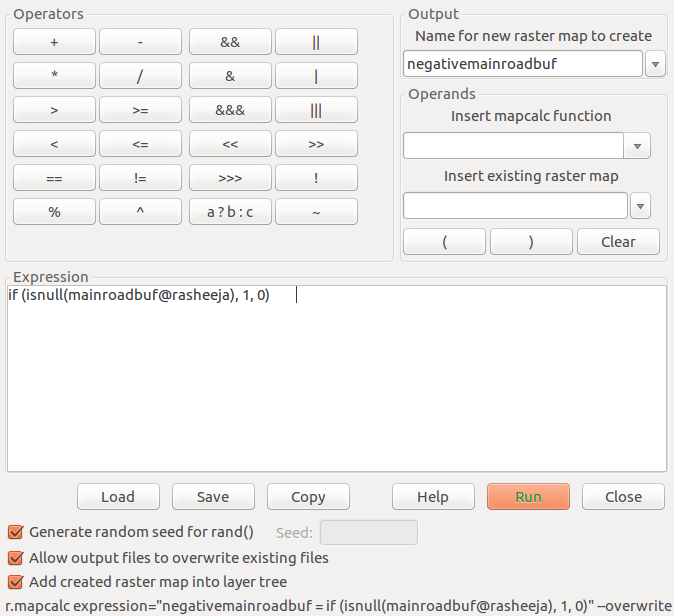
\includegraphics[width=0.7\textwidth]{pictures/reclassMainRoad.png}
  \caption{Using reclass to create a map layer which only stores main roads}
  \label{fig:reclassMainRoad}
\end{figure}

\begin{figure}[H]
  \centering
  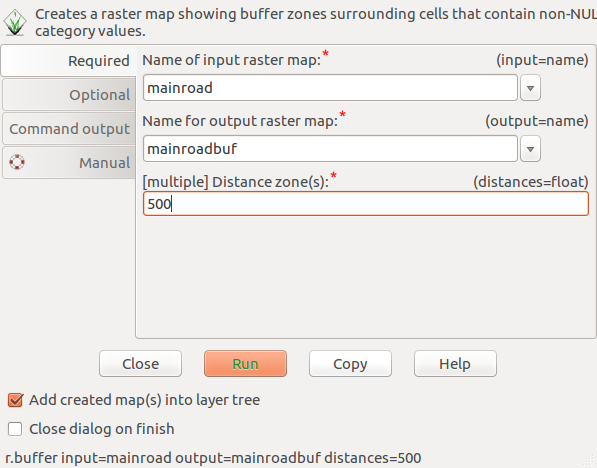
\includegraphics[width=0.7\textwidth]{pictures/bufferMainRoad.png}
  \caption{Using buffer to create a 500 unit buffer around the main roads}
  \label{fig:bufferMainRoad}
\end{figure}

\begin{figure}[H]
  \centering
  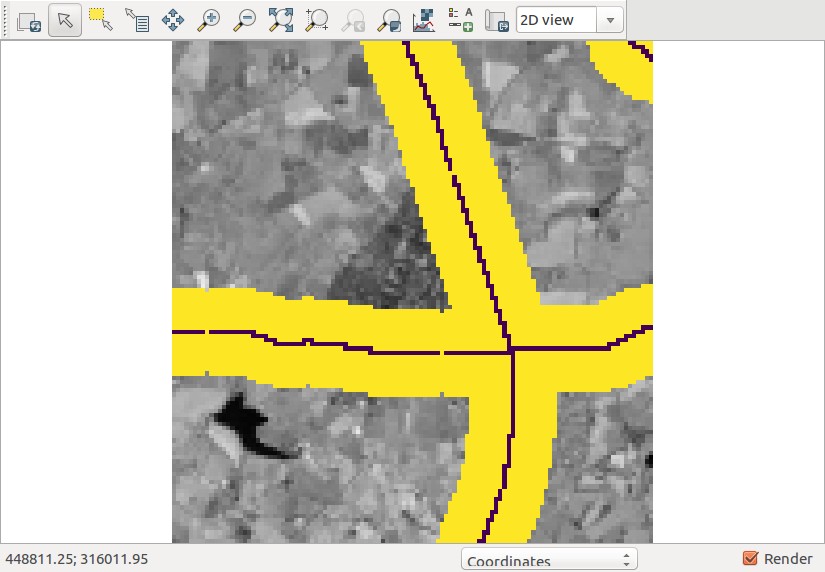
\includegraphics[width=0.7\textwidth]{pictures/bufferMainRoadMap.png}
  \caption{What the buffered map layer looks like when put on top of the image map layer}
  \label{fig:bufferMainRoadMap}
\end{figure}

From the figures shown above, it can clearly be seen how we can use buffers to create zones on the map
where it may be desirable or even undesirable for a supermarket to be opened. For example, create a
desirable buffer around a high income population, and create an undesirable buffer around areas with
lots of wildlife.

\subsubsection{Reclass}

The reclass function, when applied on a raster map, reclassifies the category layers on the raster map
depending on rules specified by the user. This reclassified map can then optionally be saved with a
given title \parencite{manualReclass}.

Reclass will be used to extract the type of features that we are interested in from a map layer and then
save it so that the extracted features can be further analysed. In Figure ~\ref{fig:reclassMainRoad}, you can
see how reclass was used to create a layer around the main roads. This was achieved by using the rules parameter
of the reclass function to set the category value for all main roads to 1, and all non main roads to NULL.

\subsubsection{Mapcalc}

Mapcalc is used to perform arithmetic operations on a raster map layer. New layers can be created as a result
of these operations \parencite{manualMapcalc}.

One way we can use mapcalc is to create negative buffers. To do this, we create a normal buffer as we have
done previously, and then use mapcalc to swap the one and zero values. See Figure ~\ref{fig:mapcalcMainRoad}
to see how the mapcalc function can be used to create a negative buffer around main roads.

\begin{figure}[H]
  \centering
  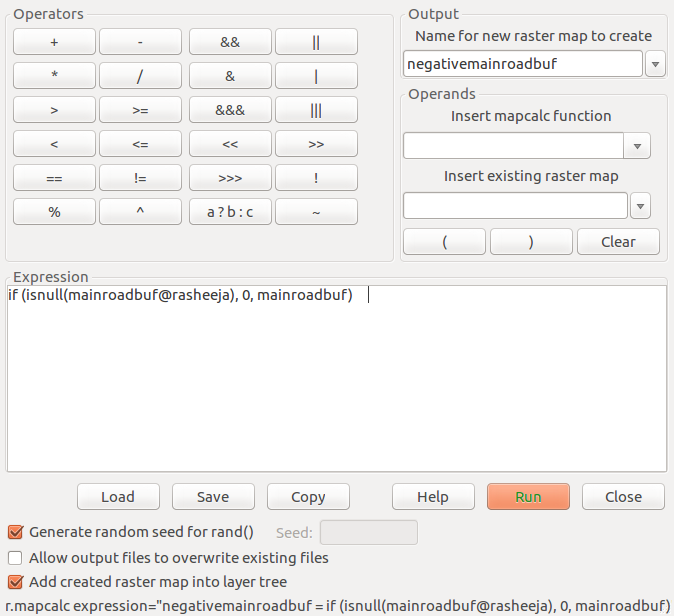
\includegraphics[width=0.7\textwidth]{pictures/mapcalcMainRoad.png}
  \caption{Mapcalc settings to create a negative buffer around main roads}
  \label{fig:mapcalcMainRoad}
\end{figure}


\begin{figure}[H]
  \centering
  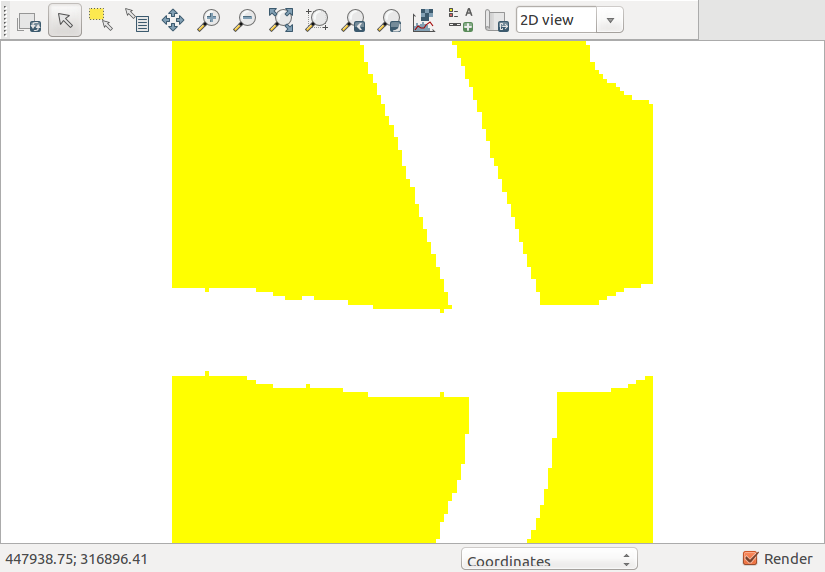
\includegraphics[width=0.7\textwidth]{pictures/negativeMainRoadBuf.png}
  \caption{Negative buffer around main roads}
  \label{fig:negativeBufferMainRoadMap}
\end{figure}

\section{Requirements}

In this section, we will go through the requirements that were given to us by Ocset and give our understanding
of these requirements. We will then discuss the information layers that are available to us and how we will
use these information layers to achieve our goal.

\subsection{The Task}
Oscet would like to open a new supermarket in the Leicestershire area and have asked us to find the best location
for the supermarket using GIS. Oscet as a company have some philosophies that they would like to adhere to. Oscet's
unique selling point is that they source their organic products from local farms. This means that their new
site either needs to be near arable land or near the local farmers to ensure that their organic food is source locally.
Oscet would also like to ensure that they do not damage the local environment so the new supermarket must not be
opened anywhere near the habitats of endangered wildlife. Finally, Oscet encourages their customers to use public
transport, so we should find the new site near some bus/train stations or withing walking distance of local populations.
If this cannot be done, Oscet will provide a bus service to their store.

There are a few more things to consider apart from Oscet's philosophies. The new supermarket will include a carpark so
the new site must have adequate space to accomodate this carpark. Oscet would also like to maximise their
profits while adhering to their philosophies, so it may be worth opening the store away from any competition and
near populations of high income.

\section{Design and Implementation}

\section{Conclusion}

\pagebreak

\printbibliography

\end{document}
